\chapter{Modi di guida d'onda rettangolare} 

\begin{figure}[h]
    \centering
    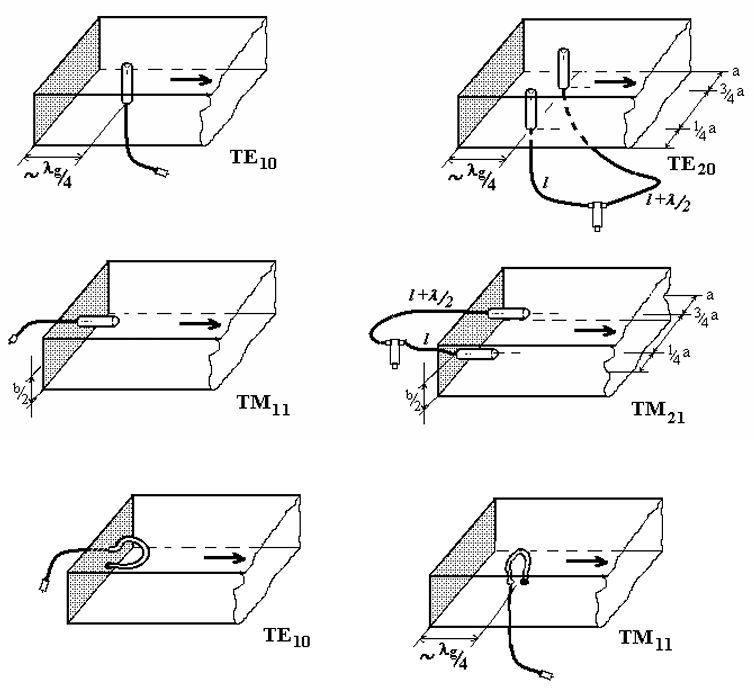
\includegraphics[scale = 0.9]{Modi di guida rettangolare.PNG}
\end{figure}  

\newpage 

\section{Modo fondamentale: $TE_{10}$}

\footnote{Slide del prof | PPT: Lezione 21 - 22 Guide rettangolari 22-24 maggio 2023 | Pag 13-20 \\ 
FWC - pag 422 \\
FWC - 8.8 The $TE_{10}$ wave in a rectangular guide - pag 423 \\
Ricevimento con prof}

\begin{tcolorbox}
    $TE_{10}$ si legge TE uno zero, non TE dieci, si legge cifra per cifra
\end{tcolorbox}

Le guide d'onda, come scritto precedentemente, possono essere $TM_{n, m}$ o $TE_{n, m}$ e variano in base ai parametri n e m. \\ 

$TE_{10}$, o detto anche modo fondamentale, è il modo di guida d'onda per cui la frequenza di taglio è minore rispetto alle altre modalità. \\ 

In formule: 

{
    \Large 
    \begin{equation}
        f_{c_{10}} = \frac{c}{2} \frac{1}{a} = \frac{1}{2 a \sqrt{\mu \varepsilon}}
    \end{equation} 
}

\begin{tcolorbox}
    Dal ricevimento con il prof: \\ \\ 

    Data la banda delle frequenze operative (cioè quelle che vogliamo trasmettere nel sistema guida d'onda), 
chiamata anche finestra: 

{
    \Large
    \begin{equation}
        B = [f_1, f_2]
    \end{equation}
} 

possiamo progettare le dimensioni della sezione della guida d'onda. \\ 

$f_2$ possiamo esprimerla anche come: 
{
    \Large
    \begin{equation}
        f_2 = \frac{f_2}{f_1} \cdot f_1 = k \cdot f_1
    \end{equation}
}
Se B è minore dell'intervallo di monomodalità, generalmente, 
è preferibile calcolare, dato B, la sezione di guida d'onda più grande possibile. \\

Coincidiamo l'estremo superiore della finestra con l'estremo superiore della banda di monomodalità, 
cosicchè le perdite sono più basse possibili perchè la finestra è più lontana 
possibile dalla frequenza di cut-off, ricordando più si avvicina alla frequenza di cut-off e maggiori sono le perdite. \\ 

Quindi: 

{
    \Large
    \begin{equation}
        f_2 [GHz] = \frac{300}{a [mm]} 
        \Rightarrow 
        a [mm] = \frac{300}{f_2 [GHz]} 
        = \frac{300}{k \cdot f_1 [GHz]}
    \end{equation}
}

e poi: 

{
    \Large 
    \begin{equation}
        b = \frac{1}{2} a 
    \end{equation}
}


\end{tcolorbox}

\begin{figure}[h]
    \centering
    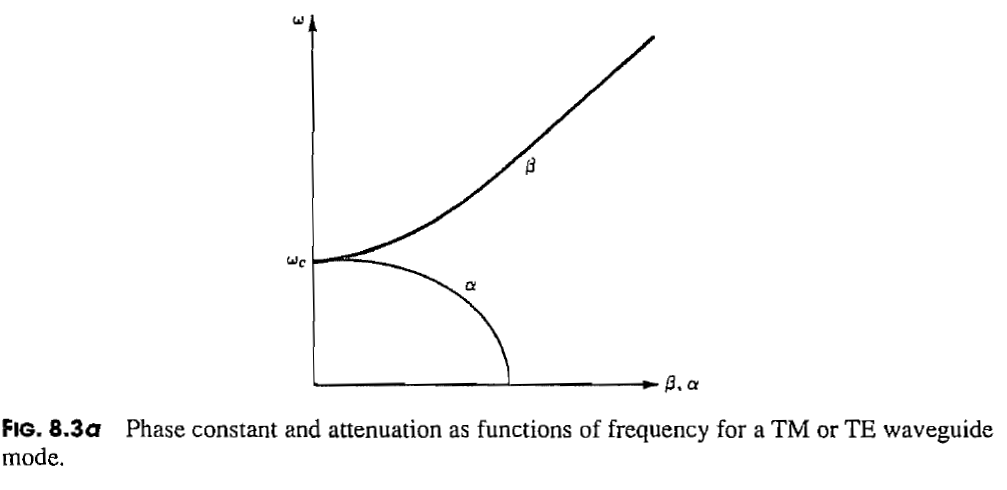
\includegraphics[scale = 0.7]{Phase constant and attenuation in parallel waveguide.PNG}
\end{figure}  

\footnote{FWE - pag 401}

\begin{tcolorbox}
    Scritto in un'altra maniera, l'onda deve essere larga almeno $\frac{\lambda}{2}$, 
    sennò non c'è propagazione. \\
    Per approfondire: \\ 
    \url{https://www.ariparma.it/risorse/articoli/Guida%20di%20onda.pdf} 
        
\end{tcolorbox}

\begin{figure}[h]
    \centering
    \includegraphics{Frequenze di cut-off in base alla modalità della guida d'onda.PNG}
\end{figure}  


La figura indica le frequenze di cut-off di diversi modi di guida d'onda. \\ 
Tipicamente, nella $TE_{10}$: 

{
    \Large
    \begin{equation}
        \frac{b}{a} = \frac{1}{2}
    \end{equation}
}

che è il valore tipicamente utilizzato nella realtà. \\ 
Normalmente, questo tipo d'onda è progettata in modo tala che la frequenza di cut-off sia il 30 per cento sotto la frequenza operativa. \\ 
In questo modo, solo un tipo d'onda si può propagare nella guida d'onda. \\ 

\begin{figure}[h]
    \centering
    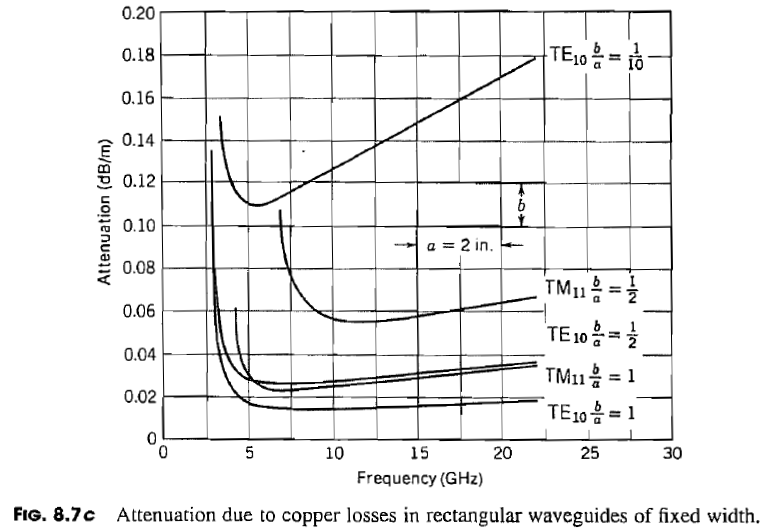
\includegraphics[scale = 0.8]{Atenuanzioni di guida d'onda con rame.PNG}
\end{figure}  



Non essendo troppo vicino alla frequenza di taglio, 
le dispersioni causate da diverse velocità di gruppo per diversi componenti di frequenze vengono minimizzati.  \\ 

Inoltre, nel modo fondamentale, la polarizzazione dei campi è fissa, 
il campo elettrico passa dal basso all'alto della guida. \\
Questa polarizzazione potrebbe essere necessaria per qualche applicazione. \\

Generalmente, viene impegato il rame come componente per le guide d'onde, e data una frequenza, l'attenuazione non è eccessivamente bassa 
rispetto a guide di altre dimensioni. \\

Nel modo fondamentale, il campo EM è il seguente: 

{
    \Large
    \begin{equation}
        \begin{cases}
            E_x = H_y = E_z = 0 \\ \\
            H_x ^{\pm} = \frac{\jmath}{\kappa_c ^{2}} \frac{\pi}{a} \beta A_{10} \sin(\frac{\pi}{a}) x e^{-\mp \jmath \beta z} \\ \\
            E_y ^{\pm} = - \frac{\jmath}{\kappa_c ^{2}} \omega \mu \frac{\pi}{a} A_{10} \sin(\frac{\pi}{a}) x e^{-\mp \jmath \beta z} 
        \end{cases}
    \end{equation}
}

in cui: 

{
    \Large 
    \begin{equation}
        \beta = \sqrt{\kappa ^{2} - (\frac{\pi}{a})^{2}}
    \end{equation}
} 

L'impedenza d'onda è uguale a: 

{
    \Large 
    \begin{equation}
        \begin{split}
            Z_{TE_{10}} 
            &= 
            - \frac{E_y}{H_x} 
            \\ 
            &= 
            \frac{\omega \mu_o}{\beta}
            \\ 
            &= 
            \frac{\omega \mu_o}{\sqrt{\kappa ^{2} - (\frac{\pi}{a})^{2}}}
        \end{split}
    \end{equation}
} 

Dal Teorema di Poynting, il flusso di potenza attiva media è:
{
    \Large
    \begin{equation}
        \begin{split}
            P_{10} 
            &= \frac{1}{2} \Re [\int_{0}^{a} \int_{0}^{b} \vec{E} \times \vec{H} ^{*} \hat{z} dx dy]
            \\ 
            &= \frac{1}{2} \Re [\int_{0}^{a} \int_{0}^{b} E_y H_x ^{*} \cdot \hat{z} dx dy]
            \\ 
            &= \frac{\omega \mu a^{3} b}{4 \pi ^{2}} \left|A_{10}\right| ^{2} \Re(\beta) 
            \\ 
            &= 
            \frac{\beta}{\omega \mu_o} \frac{\left|V^{+}\right|^{2}}{2}
        \end{split}
    \end{equation}
}


L'unico componente del campo elettrico è quello verticale $E_y$ che passa dall'alto al basso della guida. \\

$E_y$ è è massima al centro della guida e zero alle pareti della guida d'onda. \\
$H_x = 0$ alle due pareti e massimo al centro della guida, proprio come $E_y$. \\ 
$H_z$ è massima alle pareti e zero al centro. 

\begin{figure}[h]
    \centering
    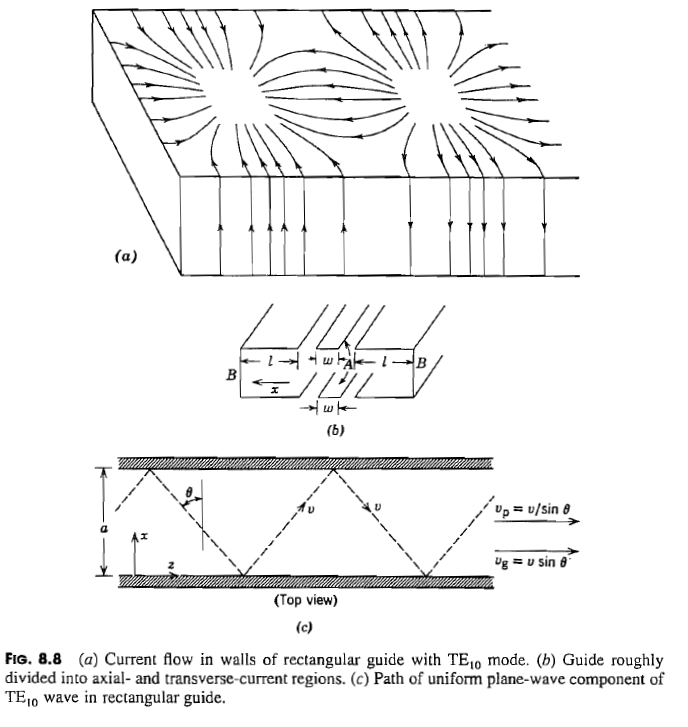
\includegraphics[scale= 0.9]{TE 10.PNG}
\end{figure}  

\newpage 

\section{Modo $TE_{20}$} 

\footnote{Slide del prof | PPT: Lezione 21 - 22 Guide rettangolari 22-24 maggio 2023 | Pag 40-42} 

Le guide d'onda sono dimensionate in modo tale che, alla frequenza di lavoro, 
ci sia solo un solo modo di propagazione, quindi: 

{
    \Large
    \begin{equation}
        a \ge 2b
    \end{equation}
}

La frequenza di cut-off per la $TE_{20}$ è: 

{
    \Large 
    \begin{equation}
        f_{c_{20}} [GHz] = \frac{300}{a [mm]}
    \end{equation}
}

Quindi l'intervallo di monomodalità, cioè l'intervallo di frequenze in cui l'onda si può propagare 
nel sistema guida d'onda così progettato è di: 

{
    \Large 
    \begin{equation}
        \frac{300}{a [mm]} \ge f[GHz] \ge \frac{150}{a [mm]}
    \end{equation}
} 

Se $m=0$, la guida d'onda non dipende da b. \\ 

$\omega_{c_{n0}}$ aumenta al diminuire di b. \\ 

Quindi b può essere il più piccolopossibile. \\ 

Ma il campo max è inversamente proporzionale a $\sqrt{b}$ 

{
    \Large 
    \begin{equation}
        \alpha_c \approx 
        \frac{R_s}{a^{3} b \kappa \eta} (2b\pi^{2} + a^{3} \kappa^{2})
    \end{equation}
}

dove: 

{
    \Large 
    \begin{equation}
        R_s = \frac{1}{\sigma \delta}
    \end{equation}
}


Quindi tipicamente: 

{
    \Large
    \begin{equation}
        a \approx 2b
    \end{equation}
}

\newpage 
